\section{Methodology}
\label{b2:methodology}

To achieve our overarching goal, the team will pursue three core components that will be the foundational basis to our new automated reasoning architecture.
Our efforts will culminate in the forth objective, which will integrate these elements and connect the results to software verification.
A baseline for each of the three core component exists in prior art, but we will pursue better methods to obtain better performance and scalability in view of the wholistic approach described above.
An improvement in one of the core components will boost the power of the resulting software verifier.
We will used standard verification benchmarks and additional benchmark suites that we construct, to gauge the quality of our core contributions.


\subsection{Bridging equality reasoning}

Equality is a fundamental concept in mathematics.
The most basic algebraic structures, such as groups,
are models (in the logical sense) of a set of equational
axioms, the likeness of $x\cdot(y\cdot z) = (x\cdot y)\cdot z$ and $x\cdot 1 = 1\cdot x = x$.
Equality is crucial for automated reasoning, because it means that mathematical objects can have more than one name --- multiple terms may represent the same object.
An inference rule $\infruleshort{K}{P(x),Q(x)}{R(x, x+1)}$
can be applied to derive a goal such as $R(y+z, y+z+1)$,
by instantiating $x\mapsto y+z$;
but it cannot be applied directly to a goal such as
$R(y+1, y+2)$, because it does not (syntactically) match the conclusion pattern $R(x,x+1)$.
The goal first has to be rephrased as the two subgoals
$y + 2 = (y + 1) + 1, R(y+1, (y+1)+1)$, using the so-called \emph{paramodulation} rule%
~\cite{Book2001:Nieuwenhuis},
at which point $K$ can be applied to the second subgoal.
The first subgoal is proved independently using an appropriate axiomatization of the integers.

The paramodulation rule is powerful as it allows the prover to subsitute any term $t_1$ with any other term $t_2$, provided that it can then prove the conjecture $t_1 = t_2$.
This is an extremely useful utility for marking progress in a given proof, but is disastrous from an automated proof search perspective:
Because it can be instantiated with \emph{any} two terms, it opens up an infinite space of possible derivations for any given goal.
Even with an efficient procedure that can find all the possible terms that are equivalent to $t_2$ (and in most cases, such procedure is not available) ---
there would still be infinitely many such terms in any non-trivial theory (for instance, $x = x + 0 = x + 0 + 0 = \cdots$).
Careful choice of where and when to apply equality reasoning is essential for effective proof search.

Superposition calculus~\cite{JACM1965:Robinson,IJCM1965:Robinson} aims to provide such control over applications of paramodulation
by imposing a \emph{simplification order} $\succ$ over the set of possible terms, and then applying \emph{term rewriting}, replacing $t_1$ by $t_2$ only when $t_1\succ t_2$.
For such a strategy to be effective, $\succ$ must be \emph{confluent}, \ie, if $t\succeq s_1,s_2$, then there
exists $t'$ such that $s_1,s_2 \succeq t'$ (where $t$, $s_{1,2}$, $t'$ are all equivalent).
Otherwise, rewriting may cause proof goals to diverge to
a state where terms occurring in them can no longer be unified via equality reasoning even though they are equivalent.
The widespread solution for constructing such an ordering is to collect the set of all known (universally quantifier) equalities $\Eqs$ and provide them as input to the Knuth-Bendix completion algorithm~\cite{AR1983:Knuth}.
The result is a \emph{directed term rewriting system} that is \emph{normalizing}, that is, any two terms $t_{1,2}$ such that $\Eqs\vdash t_1=t_2$
have a common normal form.
This is done by \emph{orienting} each $x=y \in \Eqs$ to either $x\rwto y$ or $y\rwto x$ based on a Knuth-Bendix ordering of the terms.
(In fact, the ordering is a parameter of the completion algorithm and can be configured.)
It follows that it is sufficient to reduce all the terms in the proof to their normal forms, and then any two equivalent terms will be syntactically equal.

What separates superposition calculus from an ideal solution for equational reasoning is the fact that Knuth-Bendix completion is, in reality, a \emph{semi-algorithm}:
It is not guaranteed to yield a normalizing direction for any set of equations.
Indeed, some inputs exist for which there is no such orientation of the equations.
The problem of telling whether or not a solution exists is itself undecidable (because checking even a TRS for confluence is undecidable).
One glaring situation is the case of the commutative axiom, $x\cdot y = y\cdot x$, where both orientations are equivalent and immediately cause divergence,
leading to the need of instating a side condition $x\succ y$ that arbitatily chooses one order of the operands over the other.
Fine-tuning the term ordering can have drastic effects on whether the Knuth-Bendix algorithm succeeds~\cite{ICRTA2006:Wehrman}.

Equality reasoning in SMT solvers is based on an equality theory solver that uses \emph{congruence closure} to identify (ground) terms that whose equality follows from known (quantifer-free) equality conjectures and from the equality axioms~\cite{JACM1980:Nelson}.
An efficient implementation is achieved through use of \emph{equality graphs} --- \emph{e-graphs} --- that allow fast computation of congruence closure~\cite{Thesis1980:Nelson}.
E-graphs where also in the core of one of the earlier ATPs, Simplify~\cite{JACM2005:Detlefs},
which in retrospect is now referred to as SMT.

\begin{proposal}E-graphs are a suitable formalism to serve as the bridge that unifies equality reasoning in SMT and ATP.
\end{proposal}

We propose to build a framework for equality reasoning based on e-graphs and term rewriting systems (TRSs), 
inspired by similar uses that came up in compiler optimizations and program synthesis~\cite{everything-zack}.
We will use \emph{egg}~\cite{egg}, a collection of state-of-the-art algorithms for manipulating e-graphs and for fast rewriting over the e-graph representation.
In an e-graph, terms are grouped in equivalence classes (e-classes), and shared sub-terms are not duplicated, leading to a very compact representation.
The use of TRSs provides a way to handle universally-quantified equality statements such as $\forall x,y,z.~ x\cdot(y\cdot z) = (x\cdot y)\cdot z$ and $\forall x,y.~ x\cdot y = y \cdot x$.
Previous work in compilers relied on the concept of \emph{equality saturation}~\cite{equsat}:
That term rewriting can be applied to the e-graph until it eventually captures all possible consequences of the underlying equalities, and further applications of the rewrite rules would not contribute any new terms ---
the e-graph is \emph{saturated}.
Naturally, this cannot be achieved in all circumstances.
Our first task is therefore going to be a theoretical one, investigating the property of saturation.

\begin{researchquestion}What characterizes a TRS that is \emph{saturating}, that is, reaches saturation on any input e-graph?
\end{researchquestion}
 
This question is a lifting of the finite termination and confluence properties of TRSs when operating on standard terms.
It is trivial to see that a finitely-terminating TRS will also be saturating,
although there can be an exponential blowup in the number of steps required for termination due to exploration of all possible rewrites in the e-graph setting.
The other direction is definitely not true:
We already saw the case of $x \cdot y \rwto y\cdot x$, which is an example of a non-terminating rule.
This rule is, in fact, saturating, because any $\cdot$ term has exactly two variants.
Similarly, $x \rwto 1\cdot x$ is non-terminating, and even \emph{diverging} --- every application of it yields a new term that was not derived before ($1 \to 1\cdot 1 \to 1\cdot 1 \cdot 1 \to \cdots$);
however, thanks to the compact representation of e-classes, infinitely many terms can be represented in a single, finite e-graph, so this rule is also saturating.
This is not to say that all RTSs are saturating w.r.t.\@ e-graphs.
What makes some RTSs saturating while others diverge?
Can we define classes of saturating RTSs?
Is the problem of checking saturation decidable?
Solutions to these theoretical problems will be valuable for the more practical aspects of this project,
and guide design of appropriate algorithms and approximations.

\begin{researchquestion}How can e-graphs be used in concert with propositional reasoning, to handle proof goals with arbitrary Boolean structure?
\end{researchquestion}

In SMT solvers, integration with an underlying SAT procedure is a core characteristic.
We will attempt to facilitate this form of integration for equality reasoning based on e-graphs as well.
The inspiration for this line of work comes from DPLL(T) and CDCL(T), where the solver \emph{decides} on the truth value of an atomic formula whose value is not already determined by known facts, and attempts to complete a model of the entire formula.
If that attempt fails, the solver rolls back to the point where the decision is made, now assuming the opposite.
Choosing where in the decision tree to roll back to and what information can be added when a contradiction is detected is what differentiates various solver designs.

Boolean connectives, especially logical implications, are ubiquituous in reasoning about computer programs, as they are used to model conditional control flow.
This is one of the things that brought SMT its popularity in model checking and software verification.
The e-graph structure, however is essentially \emph{flat}: Vertices are grouped into classes, but classes cannot be further composed, and they all exist on a single layer.
Boolean expressions can be represented directly, by treating the connectives as operators $\{t,f\}^k\to\{t,f\}$, but this encoding is not conducive to automated reasoning strategies, such as resolution~\cite{resolution-things?}.
In particular, \emph{case splitting}, a very basic proof technique, is computationally hard to perform, because it requires forking the computation, essentially duplicating the e-graph for each of the cases in the proof.
When searching for proofs a prover may be required to try several different split points, and doing so repeatedly is prohibitively expensive.

We introduce the novel notion of \emph{conditional conjectures} into the area of e-graphs.
This allows parts of the e-graph to be treated as \emph{subordinate}, in the sense that the facts they represent are valid under some set of assumptions.

%\subsection{Unification Modulo Theories}

\begin{researchquestion}(Unification Modulo Theories) How can equality reasoning enhance existing proof search mechanisms, and how can it be combined with other theory solvers?
\end{researchquestion}

Theorem provers offer the flexibility that comes with customizing the logic used and its inference rules.
This makes it possible to encode high-level strategies for problem decomposition, and incorporate domain knowledge for different classes of problems.
What ATPs are not good at---in some cases, in fact, pretty bad---is
handling many different cases requiring sub-proofs,
as is the situation when, \emph{e.g.}, observing a computer program with several conditional statements.
SMT solvers, on the other hand, evolved around the SAT problem and are therefore better equipped to cope with issues of Boolean structure.

\begin{figure}
\centering
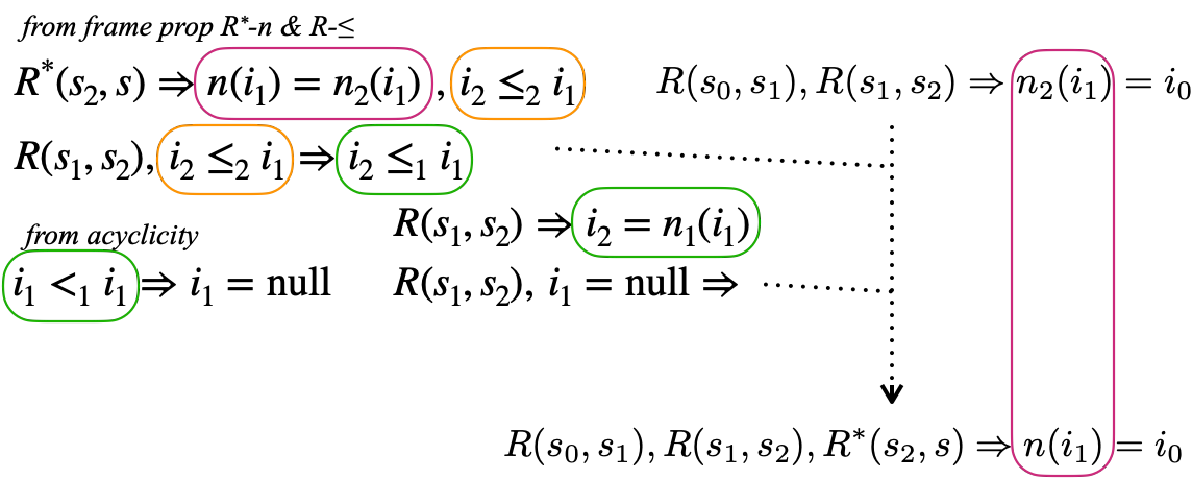
\includegraphics[width=0.65\textwidth]{img/unification-modulo-theories.pdf}
\caption{Excerpt from a correctness proof for a list reversal program, demonstrating the power of \emph{unification modulo theory}:
The bottom sequent is drived from the top-right sequent by unifying $n(i_1)$ with $n_2(i_1)$, a unification made possible by the remaining five sequents given as auxiliary assumptions.}
\label{unification:example}
\end{figure}

To facilitate effective proof search in a tool that combines the strengths of both ATP and SMT,
we propose a technique that involves dedicated theory solvers directly in the process, rather than having a narrow interface through which they communicate their results.
A core mechanism in deductive inference is that of \emph{unification}, where formulas from the goal are checked against known sequents that were previously derived to see if these sequents can fill in some pending premises.
Since both the goal and the pre-existing sequents may contain free variables, this procedure is not merely checking equality, but also provides substitution and renaming of variables when needed.
The proposed development is to enhance the unifier with knownledge about background theories, such as the theory of equality, partial orders, group theory, and transitive closure (the latter described below in \todo{}).
This would allow the unifier to not only detect syntactic matches, but also consider situations where an existing formula entails a given premise according to the theory,
and also combine several facts to satisfy one such premise.

An example illustrating how this may affect proof search is given in~\autoref{unification:example}.
The current goal is the sequent
$R(s_0,s_1), R(s_1,s_2),R^*(s_2,s) \Rightarrow
n(i_1) = i_0$,
and the prover has pre-existing fact,
$R(s_0,s_1), R(s_1,s_2) \Rightarrow n_2(i_1)=i_0$.
A-priori, the sequents cannot be unified, because the goal has $n(i_1)$ on its right-hand side, whereas the assumption has $n_2(n_1)$.
Instead of giving up on using the given assumption at this point, the prover can deduce that $n(i_1)=n_2(i_1)$ and utilize the paramodulation rule to unify the terms.
Establishing $n(i_1)=n_2(i_1)$ itself requires some extra reasoning, for example, if the prover's collection of known facts contains the sequent
$R^*(s_2,s)\Rightarrow n(i_1)=n_2(i_1), i_2\leq_2 i_1$.
The precondition $R^*(s_2,s)$ is already present, luckily, on the left-hand side of the current goal;
however, the literal $i_2\leq_2 i_1$ must be eliminated from the right-hand side before the equality can be utilized.
This is a sub-task in which SMT solvers shine:
the right-hand side of the fact is essentially a disjunction, and the solver can perform a case split and eventually discover that $i_2\leq_2 i_1$ contradicts other known properties, listed below in the figure.
During this process of elimination, an acute role is played by the literals $i_2\leq_1 i_1$, $i_1<i_1$, $i_2=n_1(i_1)$ and the underlying theory of transitive closure.